	\documentclass[12]{article}%indispensable

%-----début préambule-----

\title{\LARGE\textbf{Les indispensables en mathématiques}}
\author{Loris Caruhel}
\date{22/03/2025}

% Packages utiles pour les maths
\usepackage{mathtools, amsmath, amssymb, amsthm, amsfonts}  % Symboles et environnements mathématiques
\usepackage[french]{babel} % Langue
\usepackage[utf8]{inputenc} % Encodage
\usepackage[T1]{fontenc} % Encodage
\usepackage{hyperref} % Pour les liens hypertexts
\usepackage{xcolor} % Couleur
\usepackage[a4paper, margin=1in]{geometry} % Ajuste les marges à 1 pouce
\usepackage{longtable}
\usepackage{graphicx} % Ajouter des images
\usepackage{float}
\usepackage{enumitem}
\usepackage{amsmath} % Pour les symboles mathématiques avancés
\usepackage{amsfonts} % Pour les polices de mathématiques
\usepackage{amssymb}  % Pour les symboles supplémentaires
\usepackage{multicol}

\usepackage{amsmath, amssymb}
\usepackage{array, multirow}
\usepackage{geometry}

% Les macros
\newcommand{\R}{\mathbb R}
\newcommand{\N}{\mathbb N}
\newcommand{\Z}{\mathbb Z}


\renewcommand{\arraystretch}{2} % Hauteur des cellules des tableaux

\setlength{\tabcolsep}{15pt} % Largeur des cellules
\setlength{\parindent}{0pt}

\setlist[itemize]{topsep=10pt, itemsep=10pt} % Ajuste les espacements des listes

% Environnement
\theoremstyle{plain}
\newtheorem{thrm}{Théorème}

\theoremstyle{definition}
\newtheorem{deff}{Définition}

\theoremstyle{remark}
\newtheorem{ex}{Exemple}
\newtheorem{rem}{Remarque}

%-----fin préambule-----

\begin{document}

\maketitle
\newpage

\large
\tableofcontents

\newpage
\section{Vocabulaires}
\subsection*{Fonction injective}

Une fonction \( f : A \to B \) est \textbf{injective} si :

\[
f(x_1) = f(x_2) \Rightarrow x_1 = x_2
\]

\begin{itemize}[label=--]
	\item Cela signifie que deux éléments différents de \( A \) ont des images différentes.
	\item Pas de doublons dans les images.
\end{itemize}

\textbf{Exemple :} \( f(x) = 2x \) est injective sur \( \mathbb{R} \).  
\( f(x) = x^2 \) ne l'est pas, car \( f(2) = f(-2) = 4 \).

\vspace{0.5cm}

\subsection*{Fonction surjective}

Une fonction \( f : A \to B \) est \textbf{surjective} si :

\[
\forall y \in B, \ \exists x \in A \text{ tel que } f(x) = y
\]

\begin{itemize}[label=--]
	\item Toutes les valeurs possibles dans \( B \) sont atteintes.
\end{itemize}

\textbf{Exemple :} \( f(x) = x^3 \) est surjective sur \( \mathbb{R} \).  
\( f(x) = e^x \) ne l'est pas sur \( \mathbb{R} \), car son image est strictement positive.

\vspace{0.5cm}

\subsection*{Fonction bijective}

Une fonction est \textbf{bijective} si elle est à la fois \textbf{injective et surjective}.

\begin{itemize}[label=--]
	\item Elle associe chaque élément de \( A \) à un unique élément de \( B \), et couvre tout \( B \).
	\item Elle possède une \textbf{fonction réciproque} \( f^{-1} \).
\end{itemize}

\textbf{Exemple :} \( f(x) = x + 3 \) est bijective sur \( \mathbb{R} \).

\vspace{0.5cm}

\subsection*{Fonction réversible}

Une fonction est \textbf{réversible} si on peut revenir en arrière, c'est-à-dire s’il existe une fonction inverse \( f^{-1} \) telle que :

\[
f^{-1}(f(x)) = x
\quad \text{et} \quad
f(f^{-1}(y)) = y
\]

\textbf{Remarque :} Une fonction est réversible si et seulement si elle est bijective.

\vspace{0.5cm}

\subsection*{Fonction différentiable}

Une fonction est \textbf{différentiable} si elle admet une dérivée, c’est-à-dire si elle est "lisse", sans saut ni point anguleux.

\textbf{Exemples :}
\begin{itemize}[label=--]
	\item \( f(x) = \sin(x) \) est différentiable partout.
	\item \( f(x) = |x| \) n'est pas différentiable en \( x = 0 \), car elle présente une pointe.
\end{itemize}


\newpage
\section{Les fractions}
\large
\begin{itemize}
	\item \textbf{Addition :} \( \boxed{\dfrac{a}{b} + \dfrac{c}{d} = \dfrac{a \times d + b \times c}{b \times d}} \)
	\item \textbf{Soustraction :} \( \dfrac{a}{b} - \dfrac{c}{d} = \dfrac{a \times d - b \times c}{b \times d} \)
	\item \textbf{Multiplication :} \( \dfrac{a}{b} \times \dfrac{c}{d} = \dfrac{a \times c}{b \times d} \)
	\item \textbf{Division :} \( \dfrac{a}{b} \div \dfrac{c}{d} = \dfrac{a}{b} \times \dfrac{d}{c} = \dfrac{a \times d}{b \times c} \)
	\item \textbf{Simplification :} \( \dfrac{a \times k}{b \times k} = \dfrac{a}{b}, \quad k \neq 0 \)
	\item \textbf{Puissance :} \( \left (\dfrac{a}{b}\right )^{n} = \dfrac{a^{n}}{b^{n}} \)
	\item \textbf{Inverse :} \( \dfrac{1}{a} = a^{-1} \)
\end{itemize}
\newpage

\section{Les puissances}
\large
\begin{itemize}
	\item \textbf{Produit :} \( \boxed{a^{n}\times a^{m} = a^{n+m}} \)
	\item \textbf{Inverse :} \( \boxed{\frac{1}{a^{n}} = a^{-n}} \)
	\item \textbf{Quotient :} \( \boxed{\frac{a^{n}}{a^{m}} = a^{n-m}} \)
	\item \textbf{Puissance d'un quotient :} \( \boxed{\left( \frac{a}{b} \right)^n = \frac{a^n}{b^n}} \)
	\item \textbf{Puissance de puissance :} \( \boxed{(a^{n})^{m}=a^{n\times m}} \)
	\item \textbf{Exposants identiques :} \( \boxed{a^{n} \times b^{n} = (ab)^{n}} \)
	\item \textbf{Exposant fractionnaire :} \( \boxed{a^{\frac{m}{n}} = \sqrt[n]{a^m}} \)
	\item Pour $n$ \textbf{impair} \( \boxed{(-a)^{n} = -a^{n}} \)
	\item Pour $n$ \textbf{pair} \( \boxed{(-a)^{n} = a^{n}} \)
	\item \( \boxed{a^{0} = 1} \)
\end{itemize}
\newpage

\section{Les identités remarquables}
\large
\subsection{Puissance 2}
\begin{itemize}
	\item \(\boxed{(a + b)^2 = a^2 + 2ab + b^2} \)
	\item \(\boxed{(a - b)^2 = a^2 - 2ab + b^2} \)
	\item \(\boxed{(a + b)(a - b) = a^2 - b^2} \)
	\item \(\boxed{a^2 + b^2 = (a + b)^2 - 2ab}\)
\end{itemize}

\subsection{Puissance 3}
\begin{itemize}
	\item \(\boxed{(a + b)^3 = a^3 + 3a^2b + 3ab^2 + b^3}\)
	\item \(\boxed{(a - b)^3 = a^3 - 3a^2b + 3ab^2 - b^3}\)
	\item \(\boxed{a^3 + b^3 = (a + b)(a^2 - ab + b^2)}\)
	\item \(\boxed{a^3 - b^3 = (a - b)(a^2 + ab + b^2)}\)
\end{itemize}
\newpage

\section{Les racines}
\large
\begin{itemize}
	\item \textbf{Produit :} \( \boxed{\sqrt{ab} = \sqrt{a} \times \sqrt{b}} \)
	\item \textbf{Quotient :} \( \boxed{\sqrt{\frac{a}{b}} = \frac{\sqrt{a}}{\sqrt{b}}} \)
	\item \textbf{Racine d'une puissance :} \( \boxed{\sqrt[n]{a^m} = a^{\frac{m}{n}}} \)
	\item \textbf{Produit de racines :} \( \boxed{\sqrt{a} \times \sqrt{b} = \sqrt{ab}} \)
	\item \textbf{Racine d'un carré parfait :} \( \boxed{\sqrt{a^2} = |a|} \)
	\item \textbf{Racine carrée de zéro :} \( \boxed{\sqrt{0} = 0} \)
	\item \textbf{Racine carrée d'un nombre négatif (complexe) :} \( \boxed{\sqrt{-a} = i \sqrt{a} \quad \text{(si \(a > 0\))}} \)
	\item \textbf{Racine carrée d'une somme :} \( \boxed{\sqrt{a + b} \neq \sqrt{a} + \sqrt{b}} \)
	\item \textbf{Limites :}
	\begin{itemize}
		\item \( \boxed{\lim\limits_{x \to 0^{+}} \sqrt{x} = 0} \)
		\item \( \boxed{\lim\limits_{x \to +\infty} \sqrt{x} = +\infty} \)
	\end{itemize}
\end{itemize}
\newpage

\section{Exponentielles et logarithme}
\large
\begin{itemize}
	\item \textbf{Produit :} \( \boxed{ln(ab) = ln(a) + ln(b)} \)
	\item \textbf{Division :} \( \boxed{ln\left (\frac{a}{b}\right ) = ln(a) - ln(b)} \)
	\item \textbf{Propriété 1 :} \( \boxed{ln(a^{n}) = nln(a)} \)
	\item \textbf{Propriété 2 :} \( \boxed{ln\left (\sqrt{a}\right ) = \frac{1}{2}ln(a)} \)
	\item \textbf{Propriété 3 :} \( \boxed{ln\left (\frac{1}{b}\right ) = -ln(b)} \)
	\item \textbf{Propriété 4 :} \( \boxed{ln(e^{x}) = x} \)
	\item \textbf{Propriété 5 :} \( \boxed{e^{ln(x)} = x} \)
	\item \textbf{Limites :}
	\begin{itemize}
		\item \( \boxed{\lim\limits_{x \to +\infty} e^{x} = +\infty} \)
		\item \( \boxed{\lim\limits_{x \to -\infty} e^{x} = 0} \)
		
		\item \( \boxed{\lim\limits_{x \to 0^{+}} ln(x) = -\infty} \)
		\item \( \boxed{\lim\limits_{x \to -\infty} ln(x) = +\infty} \)
	\end{itemize}
\end{itemize}

\newpage
\section{Trigonométrie}
\subsection{Propriétés}
\begin{figure}[h] % h = ici, t = en haut, b = en bas, p = page séparée
	\centering
	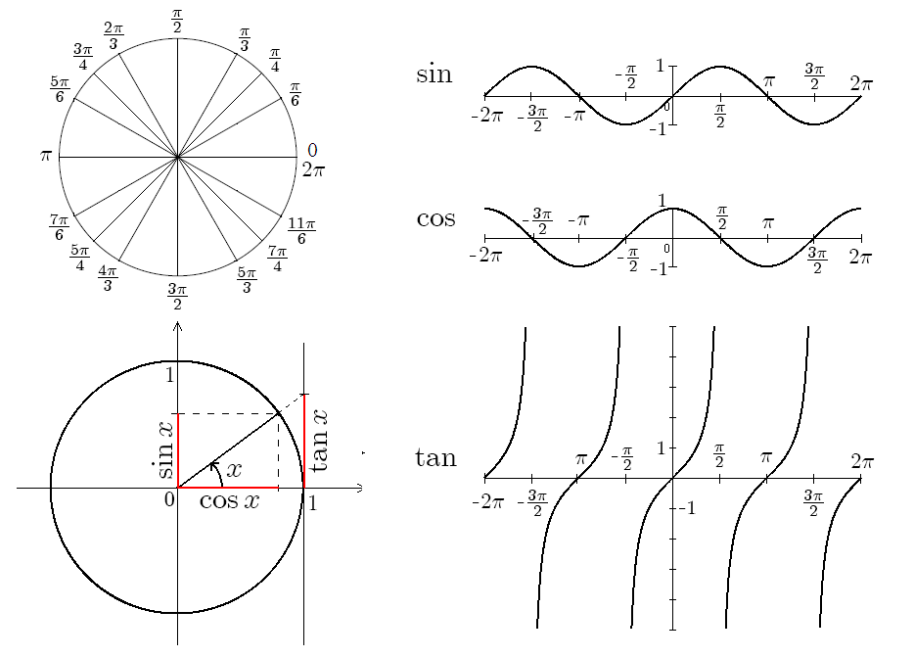
\includegraphics[width=0.8\textwidth]{./images/trigonometrie.png} % Ajustez la largeur
	\caption{Quelques propriétés des fonctions de base}
	\label{fig:trigonometrie} % Pour référencer l’image
\end{figure}

\begin{figure}[h] % h = ici, t = en haut, b = en bas, p = page séparée
	\centering
	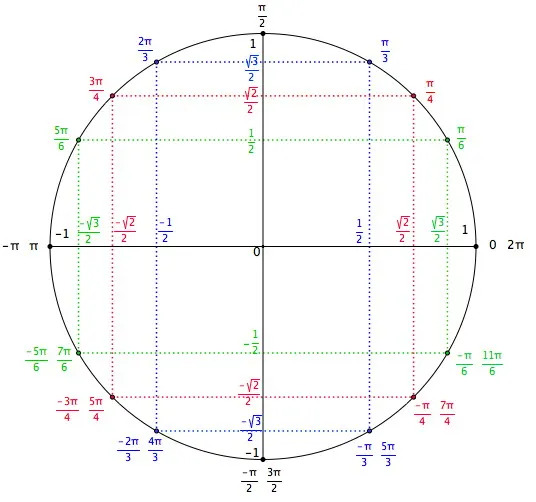
\includegraphics[width=0.5\textwidth]{./images/cercle-trigonometrique.jpg} % Ajustez la largeur
	\caption{Cercle trigonométrique}
	\label{fig:cercletrigo} % Pour référencer l’image
\end{figure}
\newpage


\subsection{Fonctions}
\subsubsection{Originales}
\begin{itemize}
	\item \( \boxed{\sin(x) = x - \frac{x^3}{3!} + \frac{x^5}{5!} - \frac{x^7}{7!} + \cdots} \)
	\item \( \boxed{\cos(x) = 1 - \frac{x^2}{2!} + \frac{x^4}{4!} - \frac{x^6}{6!} + \cdots} \)
	\item \( \boxed{\tan(x) = \frac{\sin(x)}{\cos(x)} = x + \frac{x^3}{3} + \frac{2x^5}{15} + \cdots} \quad \text{sur} \quad x \neq \frac{\pi}{2} + k\pi \quad \text{avec} \quad k \in \mathbb{Z} \)
\end{itemize}

\subsubsection{Réciproques}
\begin{itemize}
	\item \( \boxed{\arcsin(x) \quad \text{sur} \quad x \in [-1,1]} \)
	\item \( \boxed{\arccos(x) \quad \text{sur} \quad x \in [-1,1]} \)
	\item \( \boxed{\arctan(x) \quad \text{sur} \quad x \in \mathbb{R}} \)
\end{itemize}

\subsubsection{Hyperboliques}
\begin{itemize}
	\item \( \boxed{\sinh(x) = \frac{e^{x} - e^{-x}}{2}} \)
	\item \( \boxed{\cosh(x) = \frac{e^{x} + e^{-x}}{2}} \)
	\item \( \boxed{\tanh(x) = \frac{\sinh(x)}{\cosh(x)}} \)
\end{itemize}

\subsubsection{Hyperboliques réciproques}
\begin{itemize}
	\item \( \boxed{arsinh(x) = \ln\left(x + \sqrt{x^2 + 1}\right)} \)
	\item \( \boxed{arcosh(x) = \ln\left(x + \sqrt{x^2 - 1}\right)} \quad sur \quad x \geq 1 \)
	\item \( \boxed{artanh(x) = \frac{1}{2} \ln\left(\frac{1 + x}{1 - x}\right)} \quad sur \quad |x| < 1 \)
\end{itemize}

\subsubsection{Complémentaires (secondaires)}
\begin{itemize}
	\item \textbf{Cotangente :} \( \boxed{\cot(x) = \frac{1}{\tan(x)} = \frac{\cos(x)}{\sin(x)}} \quad sur \quad x \neq k\pi \)
	\item \textbf{Sécante :} \( \boxed{\sec(x) = \frac{1}{\cos(x)}} \quad sur \quad x \neq \frac{\pi}{2} + k\pi \)
	\item \textbf{Cosécante :} \( \boxed{\csc(x) = \frac{1}{\sin(x)}} \quad sur \quad x \neq k\pi \)
\end{itemize}

\subsubsection{Complémentaires hyperboliques}
\begin{itemize}
	\item \( \boxed{\coth(x) = \frac{1}{\tanh(x)} = \frac{\cosh(x)}{\sinh(x)} } \quad sur \quad x \neq 0 \)
	\item \( \boxed{sech(x) = \frac{1}{\cosh(x)}} \)
	\item \( \boxed{csch(x) = \frac{1}{\sinh(x)}} \quad sur \quad x \neq 0 \)
\end{itemize}

\subsection{Fondamentales}
\subsubsection{Identités trigonométriques fondamentales}
\begin{itemize}
	\item \( \boxed{\sin^2 x + \cos^2 x = 1} \)
	\item \( \boxed{\tan x \cdot \cot x = 1} \)
	\item \( \boxed{\tan x = \frac{\sin x}{\cos x}} \)
	\item \( \boxed{\cot x = \frac{\cos x}{\sin x}} \)
	\item \( \boxed{1 + \tan^2 x = \frac{1}{\cos^2 x}} \)
	\item \( \boxed{1 + \cot^2 x = \frac{1}{\sin^2 x}} \)
	\item \( \boxed{\sec x = \frac{1}{\cos x}} \)
	\item \( \boxed{\csc x = \frac{1}{\sin x}} \)
\end{itemize}

\subsubsection{Formules de somme et différence}
\begin{itemize}
	\item \( \boxed{\sin(a \pm b) = \sin a \cos b \pm \cos a \sin b} \)
	\item \( \boxed{\cos(a \pm b) = \cos a \cos b \mp \sin a \sin b} \)
	\item \( \boxed{\tan(a \pm b) = \frac{\tan a \pm \tan b}{1 \pm \tan a \tan b}} \)
\end{itemize}

\subsubsection{Angles associés}
\begin{itemize}
	\item \( \boxed{\sin(\pi + a) = -\sin a} \)
	\item \( \boxed{\cos(\pi + a) = -\cos a} \)
	\item \( \boxed{\tan(\pi + a) = \tan a} \quad \text{pour tout } a \in \mathbb{R}, \, a \neq \frac{\pi}{2} + k\pi, \, k \in \mathbb{Z} \)
\end{itemize}
\begin{itemize}
	\item \( \boxed{\sin\left(\frac{\pi}{2} - a\right) = \cos a} \)
	\item \( \boxed{\cos\left(\frac{\pi}{2} - a\right) = \sin a} \)
	\item \( \boxed{\tan\left(\frac{\pi}{2} - a\right) = \cot a} \quad \text{pour tout } a \in \mathbb{R}, \, a \neq k\pi, \, k \in \mathbb{Z} \)
\end{itemize}

\begin{itemize}
	\item \( \boxed{\sin\left(\frac{3\pi}{2} - a\right) = -\cos a} \)
	\item \( \boxed{\cos\left(\frac{3\pi}{2} - a\right) = -\sin a} \)
	\item \( \boxed{\tan\left(\frac{3\pi}{2} - a\right) = -\cot a} \quad \text{pour tout } a \in \mathbb{R}, \, a \neq k\pi, \, k \in \mathbb{Z} \)
\end{itemize}

\subsubsection{Arguments doubles}
\begin{itemize}
	\item \( \boxed{\sin(2a) = 2 \sin a \cos a} \)
	\item \( \boxed{\cos(2a) = \cos^2 a - \sin^2 a} \)
	\item \( \boxed{\tan(2a) = \frac{2 \tan a}{1 - \tan^2 a}} \quad \text{pour tout } a \in \mathbb{R}, \, a \neq \frac{\pi}{2} + k\pi, \, k \in \mathbb{Z} \)
\end{itemize}

\subsubsection{Arguments triples}
\begin{itemize}
	\item \( \boxed{\sin(3a) = 3 \sin a - 4 \sin^3 a} \)
	\item \( \boxed{\cos(3a) = -3 \cos a + 4 \cos^3 a} \)
	\item \( \boxed{\tan(3a) = \frac{3 \tan a - \tan^3 a}{1 - 3 \tan^2 a}} \quad \text{pour tout } a \in \mathbb{R}, \, a \neq \frac{\pi}{2} + k\pi, \, k \in \mathbb{Z} \)
\end{itemize}

\subsubsection{Formules de Carnot}
\begin{itemize}
	\item \( \boxed{1 + \cos(2a) = 2 \cos^2 a} \)
	\item \( \boxed{1 - \cos(2a) = 2 \sin^2 a} \)
\end{itemize}

\subsubsection{Formules de Simpson}
\begin{itemize}
	\item \( \boxed{\cos a \cdot \cos b = \frac{1}{2} \left[ \cos(a-b) + \cos(a+b) \right]} \)
	\item \( \boxed{\sin a \cdot \sin b = \frac{1}{2} \left[ \cos(a-b) - \cos(a+b) \right]} \)
	\item \( \boxed{\sin a \cdot \cos b = \frac{1}{2} \left[ \sin(a-b) + \sin(a+b) \right]} \)
\end{itemize}

\subsubsection{Développements tangentiels}
\begin{itemize}
	\item \( \boxed{\tan(a) + \ tan(b) = \frac{\sin(a+b)}{\cos(a) \times \cos(b)}} \)
	\item \( \boxed{\tan(a) = \frac{\sin(2a)}{2\cos^{2}(a)}} \)
\end{itemize}

\newpage
\section{Les dérivés}
\subsection{Rappel du principe des dérivés}
La dérivée d’une fonction $f(x)$ représente le taux de variation de cette fonction. Elle peut être dénotée $f’(x)$ ou encore $\frac{df}{dx}$. Le calcul et l’étude de la dérivée sont des notions importantes dans l’étude des fonctions.

\begin{figure}[h] % h = ici, t = en haut, b = en bas, p = page séparée
	\centering
	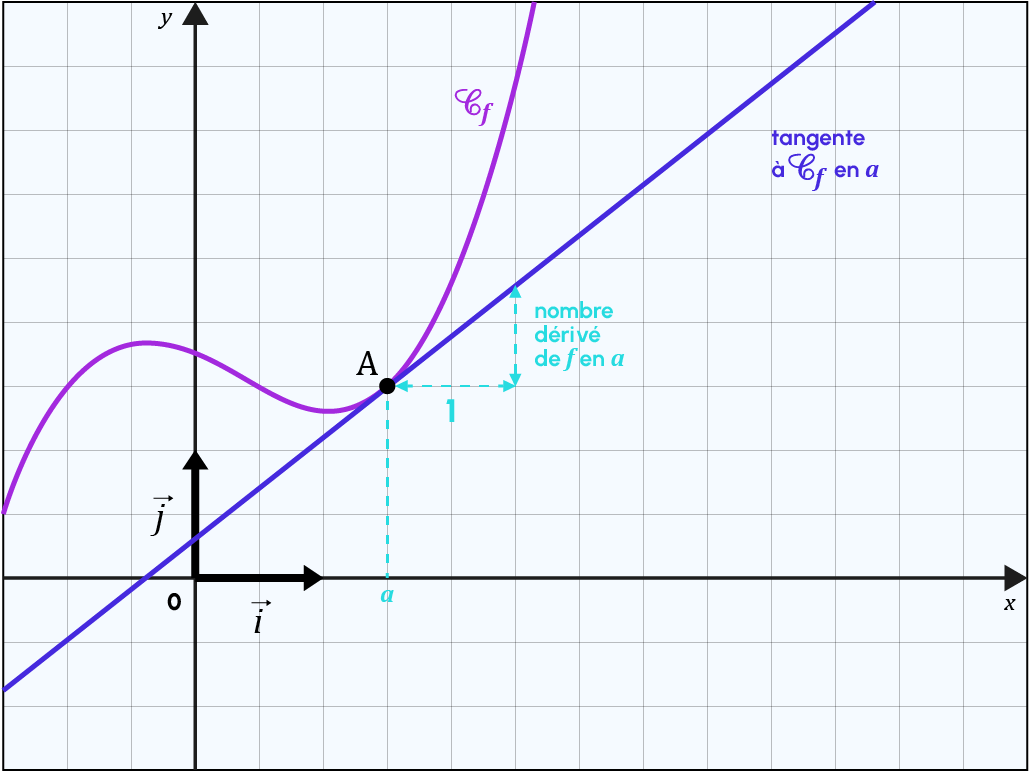
\includegraphics[width=0.5\textwidth]{./images/tangente.png} % Ajustez la largeur
	\caption{Représentation d'une tangente}
	\label{fig:tangente} % Pour référencer l’image
\end{figure}

Le signe de la dérivée permet d’indiquer les variations de la fonction $f$. C’est ce qui représente la tangente à la fonction. Et la dérivée elle-même représente le coefficient directeur de la tangente à $f$ au point. \newline

Une dérivé est représenter par le coefficient directeur de la tangente :
\begin{figure}[h] % h = ici, t = en haut, b = en bas, p = page séparée
	\centering
	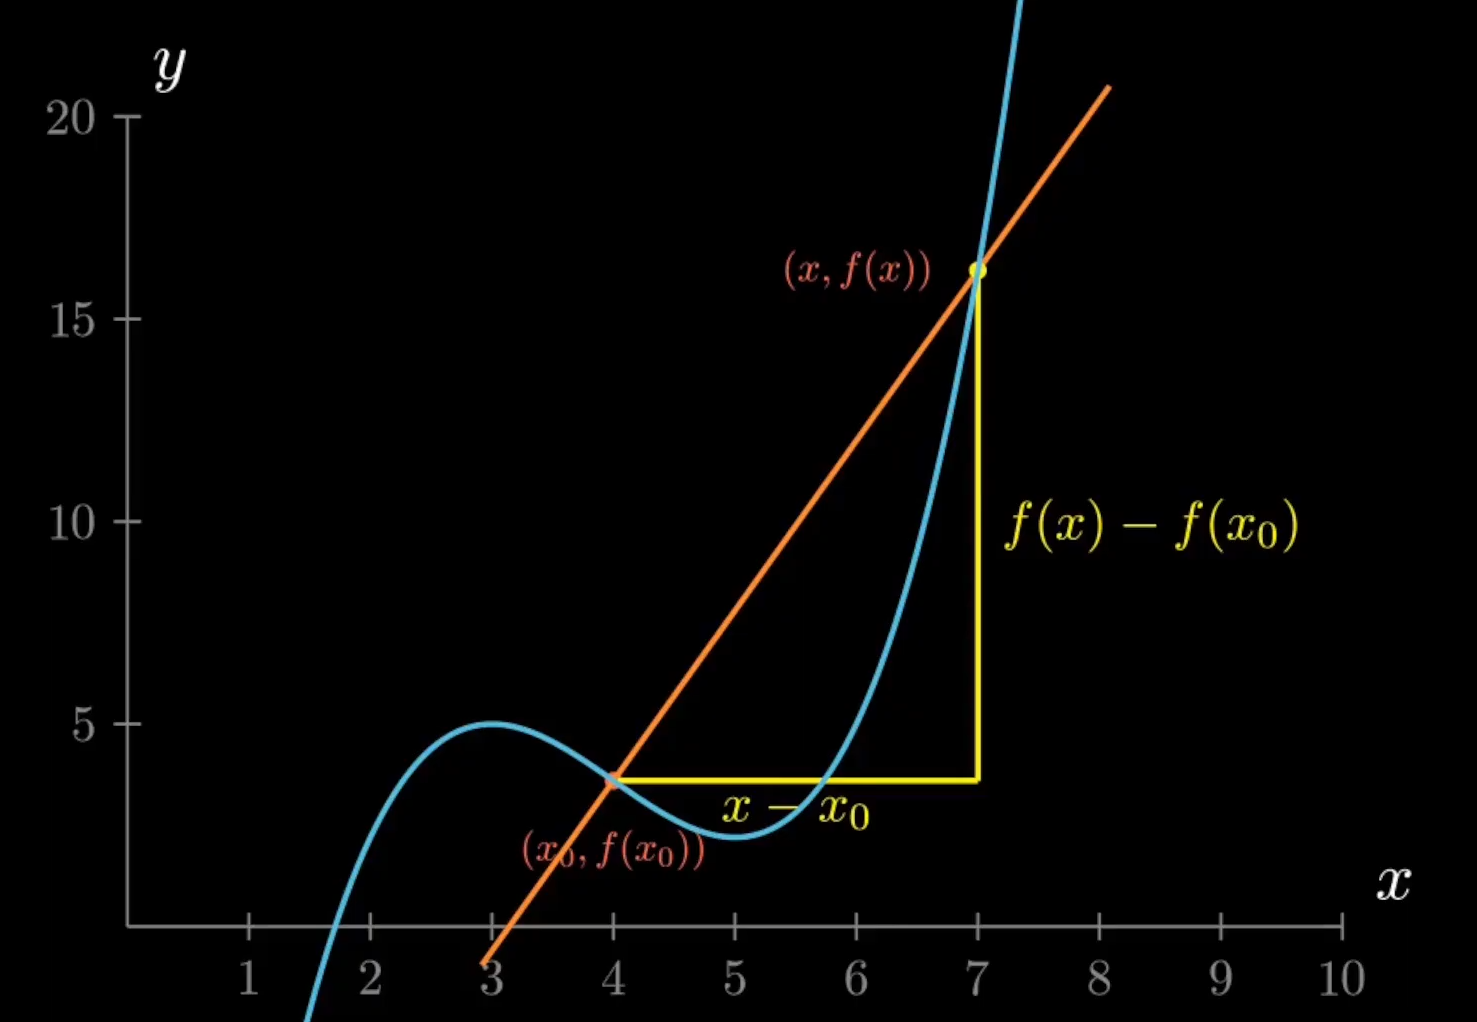
\includegraphics[width=0.5\textwidth]{./images/coef_directeur.png} % Ajustez la largeur
	\caption{Représentation du coefficient directeur}
	\label{fig:coef_directeur} % Pour référencer l’image
\end{figure}

Donc par déduction, c'est la limite de ce coefficient directeur vers le point $(x_{0}, f(x_{0}))$ \newline
Nous avons donc :
\[
\boxed{ f'(x_{0}) = \lim\limits_{x \to x_{0}} \frac{f(x)-f(x_{0})}{x-x_{0}} }
\]
Une fonction peut ne pas avoir de dérivé en tout point de celle-ci.\newline


\begin{figure}[H] % h = ici, t = en haut, b = en bas, p = page séparée
	\centering
	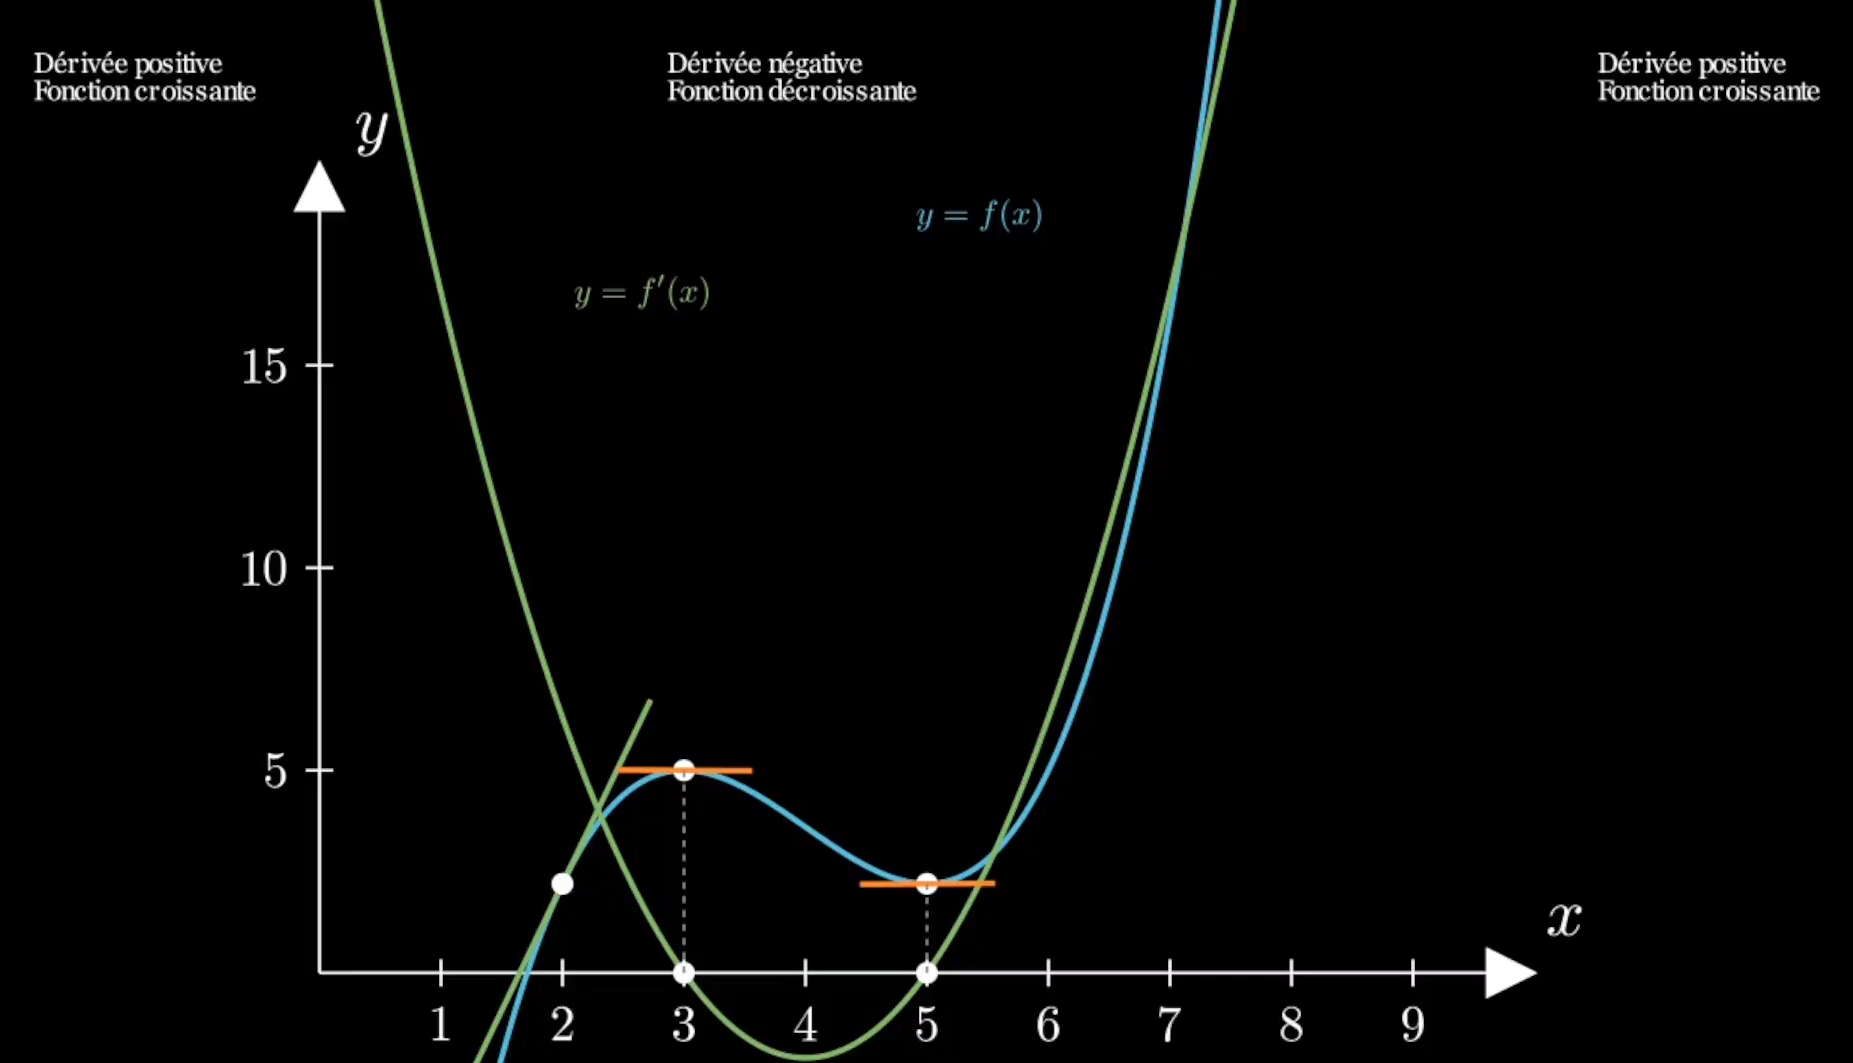
\includegraphics[width=0.5\textwidth]{./images/variations.png} % Ajustez la largeur
	\caption{Déduire le signe de la fonction}
	\label{fig:variations} % Pour référencer l’image
\end{figure}

Grâce à $f'(x)$ nous pouvons voir ici que les points où elle s'annule sont les changements de variation de la fonction $f(x)$.

\newpage
\subsection{Dérivés des fonctions usuelles}
\large
\begin{longtable}{|c|c|c|}
	\caption{Tableau des dérivés usuelles} \label{tab:derives} \\
	
	\hline
	Fonction $f$ & Dérivé $f'$ & Domaine de définition $D_f$ \\
	\hline
	\endfirsthead  % En-tête de la première page
	
	\hline
	Fonction $f$ & Dérivé $f'$ & Domaine de définition $D_f$ \\
	\hline
	\endhead  % En-tête pour les pages suivantes
	
	\hline
	\endfoot  % Pied de page pour chaque page
	
	\hline
	\endlastfoot  % Pied de page pour la dernière page
	
	% Données du tableau
	$f(x) = a$ & $f'(x) = 0$ & $\R$ \\
	$f(x) = x$ & $f'(x) = 1$ & $\R$ \\
	$f(x) = x^n$ & $f'(x) = nx^{n-1}$ & $\R, n \in \N^*$ \\
	$f(x) = \frac{1}{x}$ & $f'(x) = -\frac{1}{x^2}$ & $\left]-\infty, 0\right[ \cup \left]0, +\infty\right[$ \\
	$f(x) = \frac{1}{x^n}$ & $f'(x) = -\frac{n}{x^{n+1}}$ & $\left]-\infty, 0\right[ \cup \left]0, +\infty \right[$ \\
	$f(x) = \sqrt{x}$ & $f'(x) = \frac{1}{2\sqrt{x}}$ & $\R_+$ \\
	$f(x) = ln(x)$ & $f'(x) = \frac{1}{x}$ & $\R^*_+$ \\
	$f(x) = e^x$ & $f'(x) = e^x$ & $\R$ \\
	$f(x) = sin(x)$ & $f'(x) = cos(x)$ & $\R$ \\
	$f(x) = cos(x)$ & $f'(x) = -sin(x)$ & $\R$ \\
	$f(x) = tan(x)$ & $f'(x) = 1 + tan^2(x) = \frac{1}{cos^2(x)}$ & $\R \backslash \left\{\frac{\pi}{2}+k\pi, k \in \Z\right\} $ \\
	
	\hline
	$f(x) = u$ & $f'(x) = u'$ & $$ \\
	$f(x) = u^n$ & $f'(x) = nu'u^{n-1}$ & $$ \\
	$f(x) = \frac{1}{u}$ & $f'(x) = -\frac{u'}{u^2}$ & $$ \\
	$f(x) = \frac{1}{u^n}$ & $f'(x) = -\frac{nu'}{u^{n-1}}$ & $$ \\
	$f(x) = \sqrt{u}$ & $f'(x) = \frac{u'}{2\sqrt{u}}$ & $$ \\
	$f(x) = ln(u)$ & $f'(x) = \frac{u'}{u}$ & $$ \\
	$f(x) = e^u$ & $f'(x) = u'e^u$ & $$ \\
	$f(x) = sin(u)$ & $f'(x) = u'cos(u)$ & $$ \\
	$f(x) = cos(u)$ & $f'(x) = -u'sin(u)$ & $$ \\
	$f(x) = tan(u)$ & $f'(x) = u'(1 + tan^2(u))$ & $$ \\
	$f(x) = u+v$ & $f'(x) = u'+v'$ & $$ \\
	$f(x) = uv$ & $f'(x) = u'v + uv'$ & $$ \\
	$f(x) = \frac{u}{v}$ & $f'(x) = \frac{u'v - uv'}{v^2}$ & $$ \\
	$f(x) = au$ & $f'(x) = au'$ & $$ \\
	
	\hline
	$f(x) = (f \circ g)(x)$ & $f'(x) = g'(x)(f'(x) \circ g(x))$ & $$ \\
\end{longtable}

\newpage
\section{Les primitives usuelles}

\large
\begin{longtable}{|c|c|c|}
	\caption{Tableau des primitives usuelles} \label{tab:primitives} \\
	
	\hline
	Fonction $f$ & Primitives $F$ & Domaine de définition $D_f$ \\
	\hline
	\endfirsthead  % En-tête de la première page
	
	\hline
	Fonction $f$ & Primitives $F$ & Domaine de définition $D_f$ \\
	\hline
	\endhead  % En-tête pour les pages suivantes
	
	\hline
	\endfoot  % Pied de page pour chaque page
	
	\hline
	\endlastfoot  % Pied de page pour la dernière page
	
	% Données du tableau
	$f(x) = k$ & $F(x) = kx+C$ & $\R$ \\
	$f(x) = x$ & $F(x) = \frac{x^2}{2}$ & $\R$ \\
	$f(x) = x^n$ & $F(x) = \frac{x^{n+1}}{n+1}+C$ & $n \in \Z \backslash \left \{-1;0 \right \}$ \\
	$f(x) =a^x$ & $F(x) = \frac{a^{x}}{ln(a)}+C$ & $\R$ \\
	$f(x) = \frac{1}{x}$ & $F(x) = ln(|x|)+C$ & $\R^{*}$ \\
	$f(x) = \frac{1}{x^n}$ & $F(x) = -\frac{1}{(n-1)x^{n-1}}+C$ & $\left]-\infty, 0\right[ \cup \left]0, +\infty \right[$ \\
	$f(x) = \frac{1}{\sqrt{x}}$ & $F(x) = 2\sqrt{x}+C$ & $\R_+$ \\
	$f(x) = ln(x)$ & $F(x) = xln(x)-x+C$ & $\R^*_+$ \\
	$f(x) = e^x$ & $F(x) = e^x+C$ & $\R^*_+$ \\
	$f(x) = sin(x)$ & $F(x) = -cos(x)+C$ & $\R$ \\
	$f(x) = cos(x)$ & $F(x) = sin(x)+C$ & $\R$ \\
	$f(x) = tan(x)(x)$ & $F(x) = -ln(|cos(x)|)+C$ & $\R - \left\{ \frac{\pi}{2} + k\pi \right\}$ \\
	$f(x) = 1+tan^2(x) = \frac{1}{cos^2(x)}$ & $F(x) = tan(x)+C$ & $ \left]-\frac{\pi}{2}+k\pi, \frac{\pi}{2}+k\pi \right[, k \in \Z$ \\
	
	\hline
	$f(x) = u'u^n$ & $F(x) = \frac{u^{n+1}}{n+1}+C$ & $n \in \Z \backslash \left \{-1;0 \right \}$ \\  
	$f(x) = \frac{u'}{\sqrt{u}}$ & $F(x) = 2\sqrt{u}+C$ & $\R$ \\  
	$f(x) = \frac{u'}{u^2}$ & $F(x) = -\frac{1}{u}+C$ & $n \in \N, n \geq 2$ \\  
	$f(x) = \frac{u'}{u^n}$ & $F(x) = -\frac{1}{(n-1)u^{n-1}}+C$ & $n \in \N, n \geq 2$ \\  
	$f(x) = \frac{u'}{u}$ & $F(x) = ln(|u|)+C$ & $\R$ \\  
	$f(x) = u'e^{u}$ & $F(x) = e^{u}+C$ & $\R$ \\  
	$f(x) = u'cos(u)$ & $F(x) = sin(u)+C$ & $\R$ \\  
	$f(x) = u'sin(u)$ & $F(x) = -cos(u)+C$ & $\R$ \\  
	$f(x) = u'tan(u)$ & $F(x) = -ln | cos(u) | + C$ & $\R - \left\{ \frac{\pi}{2} + k\pi \right\}$ \\  
	
\end{longtable}

\newpage
\section{Intégrales}
\subsection{Propriétés de l'intégrale}

\[ \boxed{\int_{a}^{b} f(x)dx = -\int_{a}^{b}f(x)dx} \]
\[ \boxed{\int_{a}^{b} f(x)dx + \int_{b}^{c} f(x)dx = \int_{a}^{c} f(x)dx \quad (\text{Chasles})} \]
\[ \boxed{f(x) \geq sur [a;b] \Rightarrow \int_{a}^{b} f(x)dx \geq 0 \quad (\text{Positivité})} \]
\[ \boxed{\int_{a}^{b} (\alpha f+\beta g) = \alpha \int_{a}^{b}f + \beta \int_{a}^{b} g \quad (\text{Linéarité})} \]


\subsection{Intégration par parties}
L'intégration par parties est une méthode inspirée de la dérivation d'un produit de fonctions.

\subsection*{Formule générale}

\[
\boxed{\int u(x)\,v'(x)\,dx = u(x)\,v(x) - \int u'(x)\,v(x)\,dx}
\]

\subsection*{Justification (à partir de la dérivée d’un produit)}

On sait que :
\[
\frac{d}{dx} \left( u(x)\,v(x) \right) = u'(x)\,v(x) + u(x)\,v'(x)
\]

En intégrant des deux côtés :
\[
\int \frac{d}{dx} \left( u(x)\,v(x) \right) dx = \int u'(x)\,v(x)\,dx + \int u(x)\,v'(x)\,dx
\]

Or, par la propriété fondamentale de l'intégration :
\[
u(x)\,v(x) = \int u'(x)\,v(x)\,dx + \int u(x)\,v'(x)\,dx
\]

En isolant l'intégrale cherchée :
\[
\int u(x)\,v'(x)\,dx = u(x)\,v(x) - \int u'(x)\,v(x)\,dx
\]

\subsection*{Choix des fonctions}

On choisit :
\begin{itemize}
	\item \( u(x) \) : une fonction facile à dériver,
	\item \( v'(x) \) : une fonction facile à intégrer.
\end{itemize}

\subsection*{Exemple}

Calculons :
\[
\int x\,e^x\,dx
\]

On choisit :
\[
u(x) = x \quad \Rightarrow \quad u'(x) = 1
\]
\[
v'(x) = e^x \quad \Rightarrow \quad v(x) = e^x
\]

Alors, d'après la formule d'intégration par parties :
\[
\int x\,e^x\,dx = x\,e^x - \int 1 \cdot e^x\,dx
\]
\[
\int x\,e^x\,dx = x\,e^x - e^x + C
\]


\begin{figure}[h] % h = ici, t = en haut, b = en bas, p = page séparée
	\centering
	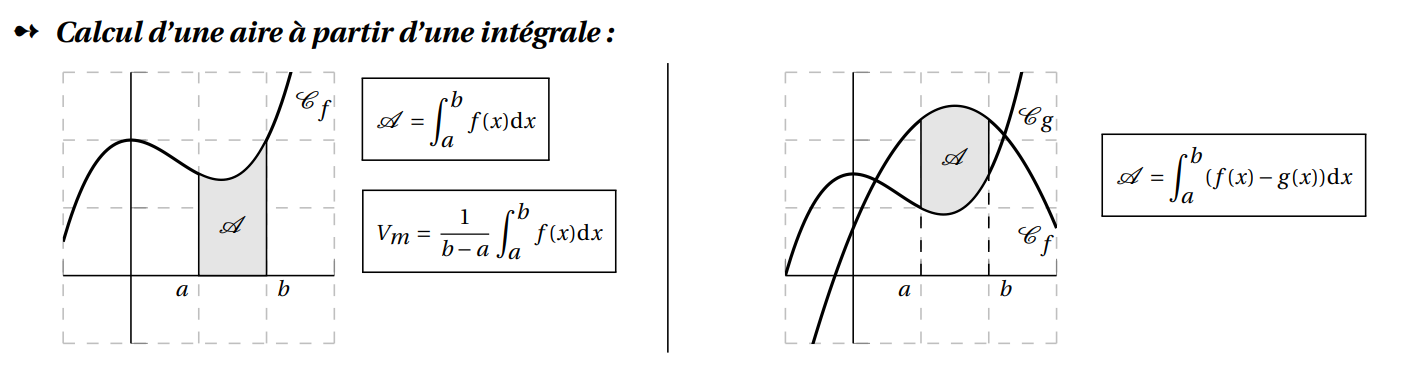
\includegraphics[width=1\textwidth]{./images/integrale.png} % Ajustez la largeur
	\caption{Calculs d'intégrales sur une courbes}
	\label{fig:integrale} % Pour référencer l’image
\end{figure}


\newpage
\section{Le changement de variable}

Le changement de variable est une méthode fondamentale utilisée en mathématiques pour simplifier une expression, résoudre une équation, ou effectuer un calcul (comme une dérivée, une intégrale, ou une équation différentielle).

\subsection*{Principe général}

On remplace une variable \( x \) par une nouvelle variable \( u \), définie par une fonction :
\[
u = \varphi(x)
\]

Cela permet de transformer un problème en fonction de \( x \) en un problème en fonction de \( u \), souvent plus simple à traiter.

\subsection*{But}

Le but est de :
\begin{itemize}
	\item simplifier une expression complexe,
	\item adapter une fonction à une forme connue,
	\item utiliser une symétrie ou une substitution astucieuse,
	\item résoudre plus facilement une équation ou une intégrale.
\end{itemize}

\subsection*{Exemple : résolution d'équation}

Résolvons l'équation suivante :
\[
x^4 + 2x^2 - 8 = 0
\]

On pose :
\[
u = x^2 \quad \Rightarrow \quad x^4 = u^2
\]

L'équation devient :
\[
u^2 + 2u - 8 = 0
\]

On résout :
\[
u = \frac{-2 \pm \sqrt{(2)^2 + 4 \cdot 8}}{2} = \frac{-2 \pm \sqrt{36}}{2} = \frac{-2 \pm 6}{2}
\Rightarrow u = 2 \text{ ou } u = -4
\]

On revient à la variable \( x \) :
\[
x^2 = 2 \Rightarrow x = \pm \sqrt{2} \qquad \text{(car } x^2 = -4 \text{ n'a pas de solution réelle)}
\]

\subsection*{Remarque}

Le changement de variable doit être :
\begin{itemize}
	\item \textbf{bijectif*} (ou du moins localement injectif*) pour être réversible*,
	\item \textbf{différentiable*} si on travaille avec des fonctions continues, dérivables ou intégrables,
	\item accompagné d'un retour à la variable initiale si nécessaire.
\end{itemize}

\newpage
\section{Limites usuelles}
	
\begin{itemize}
	\item \( \displaystyle \lim_{x \to +\infty} x^2 = +\infty \quad \lim_{x \to -\infty} x^2 = +\infty \)
	\item \( \displaystyle \lim_{x \to +\infty} x^3 = +\infty \quad \lim_{x \to -\infty} x^3 = -\infty \)
	\item \( \displaystyle \lim_{x \to +\infty} \sqrt{x} = +\infty \)
\end{itemize}


\subsection{Logarithmes et exponentielles}

\begin{itemize}
	\item \( \displaystyle \lim_{x \to 0^+} \ln x = -\infty \quad \lim_{x \to +\infty} \ln x = +\infty \)
	\item \( \displaystyle \lim_{x \to -\infty} e^x = 0 \quad \lim_{x \to +\infty} e^x = +\infty\)
\end{itemize}

\subsection{Puissances et racines}

\begin{itemize}
	\item \( \displaystyle \lim_{x \to 0^+} \frac{1}{x} = +\infty \quad \lim_{x \to 0^-} \frac{1}{x} = -\infty \)
	\item \( \displaystyle \lim_{x \to \infty} \frac{1}{x^n} = 0 \quad \text{(pour } n > 0 \text{)} \)
	\item \( \displaystyle \lim_{x \to \infty} \sqrt[x]{x} = 1 \)
\end{itemize}

\subsection{Comparaisons importantes}

\begin{itemize}
	\item \( x \ll \ln x \ll x^a \ll a^x \ll x! \ll x^x \quad \text{avec } x \to +\infty \text{ et } a > 1 \)
\end{itemize}

\subsection{Limites du type}
Faire la règle des signes
\[
\boxed{
	\begin{array}{ccc}
		\displaystyle \frac{k \ne 0}{\pm\infty} = 0^\pm &
		\quad \displaystyle \frac{k \ne 0}{0^\pm} = \pm\infty &
		\quad \displaystyle \pm \infty \times \pm \infty = \pm \infty
	\end{array}
}
\]

\subsection{Forme indéterminée (FI)}

\[
\boxed{
	\begin{array}{@{\hskip 3pt} c @{\hskip 6pt} c @{\hskip 6pt} c @{\hskip 6pt} c @{\hskip 6pt} c @{\hskip 6pt} c @{\hskip 6pt} c @{\hskip 3pt}}
		\displaystyle \frac{\infty}{\infty}  \qquad \qquad &
		\displaystyle \frac{0}{0}  \qquad \qquad &
		\displaystyle 0 \times \infty \qquad \qquad &
		\displaystyle \infty - \infty \qquad \qquad &
		\displaystyle (+\infty) + (-\infty) \qquad \qquad &
		\displaystyle 1^\infty \qquad \qquad &
		\displaystyle \infty^0 \qquad 0^0
	\end{array}
}
\]


\textit{En présence d’une FI, on peut développer, factoriser, utiliser les "croissances comparées".}

\subsection{Croissances comparées}

\begin{itemize}
	\item \( \displaystyle \lim_{x \to 0^+} x^n \ln x = 0 \)
	\item \( \displaystyle \lim_{x \to +\infty} \frac{\ln x}{x^n} = 0 \)
	\item \( \displaystyle \lim_{x \to -\infty} x^n e^x = 0 \)
	\item \( \displaystyle \lim_{x \to +\infty} \frac{e^x}{x^n} = +\infty \)
\end{itemize}

\subsection{Opérations sur les limites}
\subsubsection{Somme}
\begin{tabular}{|l|c|c|c|c|c|c|}
	\hline
	$\displaystyle \lim_{x \to \alpha} f(x) = $ & $L$ & $L$ & $L$ & $+\infty$ & $-\infty$ & $+\infty$ \\
	\hline
	$\displaystyle \lim_{x \to \alpha} g(x) = $ & $L'$ & $+\infty$ & $-\infty$ & $+\infty$ & $-\infty$ & $-\infty$ \\
	\hline
	$\displaystyle \lim_{x \to \alpha} f(x)+g(x) = $ & $L+L'$ & $+\infty$ & $-\infty$ & $+\infty$ & $-\infty$ & $F.I.$ \\
	\hline
\end{tabular}

\subsubsection{Produit}
\begin{tabular}{|l|c|c|c|c|}
	\hline
	$\displaystyle \lim_{x \to \alpha} f(x) = $ & $L$ & $L$ & $\infty$ & $0$ \\
	\hline
	$\displaystyle \lim_{x \to \alpha} g(x) = $ & $L'$ & $\infty$ & $\infty$ & $\infty$ \\
	\hline
	$\displaystyle \lim_{x \to \alpha} f(x) \times g(x) = $ & $L \times L'$ & $\infty$ & $\infty$ & $F.I.$ \\
	\hline
\end{tabular}

$\infty$ désigne $+\infty$ ou $-\infty$.

\subsubsection{Quotient}
\begin{tabular}{|l|c|c|c|c|c|c|}
	\hline
	$\displaystyle \lim_{x \to \alpha} f(x) = $ & $L$ & $L \ne 0$ & $L$ & $\infty$ & $\infty$ & $0$ \\
	\hline
	$\displaystyle \lim_{x \to \alpha} g(x) = $ & $L' \ne 0$ & $0$ & $\infty$ & $L$ & $\infty$ & $0$ \\
	\hline
	$\displaystyle \lim_{x \to \alpha} \frac{f(x)}{g(x)} = $ & $\frac{L}{L'}$ & $\infty$ & $0$ & $\infty$ & $F.I.$ & $F.I.$ \\
	\hline
\end{tabular}


\newpage
\section{Polynômes}
\subsection{Polynômes du 1er et 2ème degré}
\begin{figure}[h] % h = ici, t = en haut, b = en bas, p = page séparée
	\centering\texttt{}
	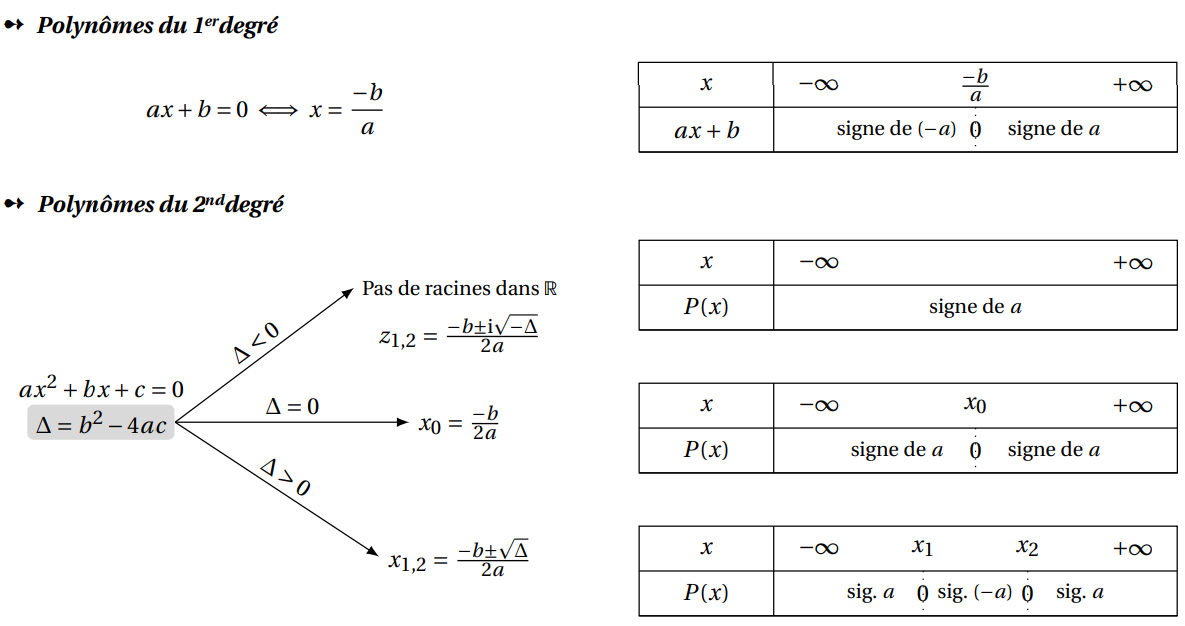
\includegraphics[width=1\textwidth]{./images/polynomes.png} % Ajustez la largeur
	\label{fig:polynome} % Pour référencer l’image
\end{figure}


\end{document}